\chapter{Concentration inequalities}
A lot of results in statistical learning is proved using bounds. For example, if $X_{1},\dots,X_n$ are independent Bernoulli $(\theta)$ random variables representing the outcomes of a sequence of $n$ tosses of a coin with bias (probability of head), then for any $\epsilon \in (0,1)$: 
\begin{equation}\label{eqs:coin_toss_bound}
    \mathbb{P} \Big(\lvert \hat{\theta}_{n} - \theta \geq \epsilon\Big) \leq 2e^{-2\epsilon^{2}}, \quad \text{for } \hat{\theta}_{n} = \frac{1}{n} \sum^{n}_{i=1} X_i
\end{equation}
For the fraction of heads in $X^n=(X_1,\dots,X_n)$. Since $\theta = \mathbb{E}\hat{\theta}_{n}$, \ref{eqs:coin_toss_bound} says that the sample (or empirical) average of $X_{i}$ concentrates sharply around the statistical average. Bound like these are fundamental in statistical learning theory (well, mostly for proof, not going to lie). For now, let us learn the technique used to derive such bounds for settings much more complicated than coin tossing. 

\section{What are concentration inequalities?}

In a probabilistic setting, we are sometimes interested of the random fluctuations of functions of independent random variables. \textit{Concentration inequalities} quantify such statements, typically by bounding the probability that such a function differs from its expected value (or from its median) by more than a certain amount. \index{concentration inequalities}

The search for concentration inequalities has been a topic of intensive research in the last decades in a variety of areas because of their importance in numerous applications. Typically, this falls into the range of designing non-deterministic (by the definition of such words), dynamic randomized algorithms or procedure of interest, while able to bound them with concentration inequalities to a certain given degree of high probabilistic `accuracy', for example. Among the areas of applications, without trying to be exhaustive, we mention statistics, learning theory, discrete mathematics, statistical mechanics, random matrix theory, information theory, and high-dimensional geometry (while not actually sure why geometry is in here). 

Informally, the \textit{concentration phenomenon} asserts that if $X_{1},\dots,X_{n}$ are independent random variables, then $f(X_{1},\dots,X_{n})$ does not deviate much from its mean provided that $f(x_{1},\dots,x_{n})$ is not too sensitive in any of its coordinate $x_{i}$. While concentration properties for sums of independent random variables were thoroughly studied and fairly well understood in classical probability theory, powerful tools to handle more general functions of independent random variables were not introduced until the appearance of \textit{martingale methods} in the 1970s, by Yurinskii (1976), Maurey (1979), Milman and Schechtman (1986), Shamir and Spencer (1987) and McDiarmid (1989). \index{martingale methods}
\begin{note}
    While the topic itself is much more complex than it is guaranteed to be, a \textit{martingale} can be defined as a sequence of random variables (i.e. for a stochastic process) for which, at a particular time, the conditional expectation of the next value in the sequence is equal to the present value, regardless of all prior values. A basic definition can be achieved. For a process $(M_n)_{n\geq 0}$, it is called martingale if:
    \begin{itemize}[noitemsep,topsep=1pt]
        \item For every $n\geq 0$, the expectation $\mathbb{E}[M_n]$ is finite, and hence equivalently, $\mathbb{E}[\lvert M_n \rvert]< \infty$.
        \item For every $n\geq 0$ and all $m_{n},m_{n-1},\dots,m_{0}$ we have: \begin{equation}
            \mathbb{E}(M_{n+1}\mid M_n = m_{n},\dots, M_{0}=m_{0}) = m_{n}
        \end{equation}
    \end{itemize} 
\end{note}

\section{Basic tools}
Of our book chapter, by a \textit{concentration inequality} we most often mean an upper bound for the probability that a real-valued random variable $Z$ differs from its expected value by more than a certain amount. In other word, we seek upper bounds for tail probabilities of the form 
\begin{equation}
    \mathbb{P}[Z-\mathbb{E}(Z)\geq t], \quad \mathbb{P}[Z-\mathbb{E}(Z)\leq -t] 
\end{equation}
where $t>0$. Of course, here we assume implicitly that the expected value exists, as for the probability to be included of the measurable space. 

To derive a lot of our concentration bounds that will solve such problem, however, we have to develop a few basic tools in the analysis. This will include Markov's inequality, Chebyshev's inequality, the Chernoff bound (often called the Chernoff trick), and Hoeffding's lemma. 
\subsection{Markov's inequality}
Let $Y\in \mathbb{R}$ be a nonnegative random variable. Then for any $t> 0$, we have the \textit{Markov's inequality} \index{Markov's inequality}: 
\begin{equation}
    \mathbb{P}(Y\geq t) \leq \frac{\mathbb{E}[Y]}{t}
\end{equation}
Before jumping straight into a proof, let us see what are we looking at from the perspective of the inequality.
\begin{figure}[h!]
    \centering
    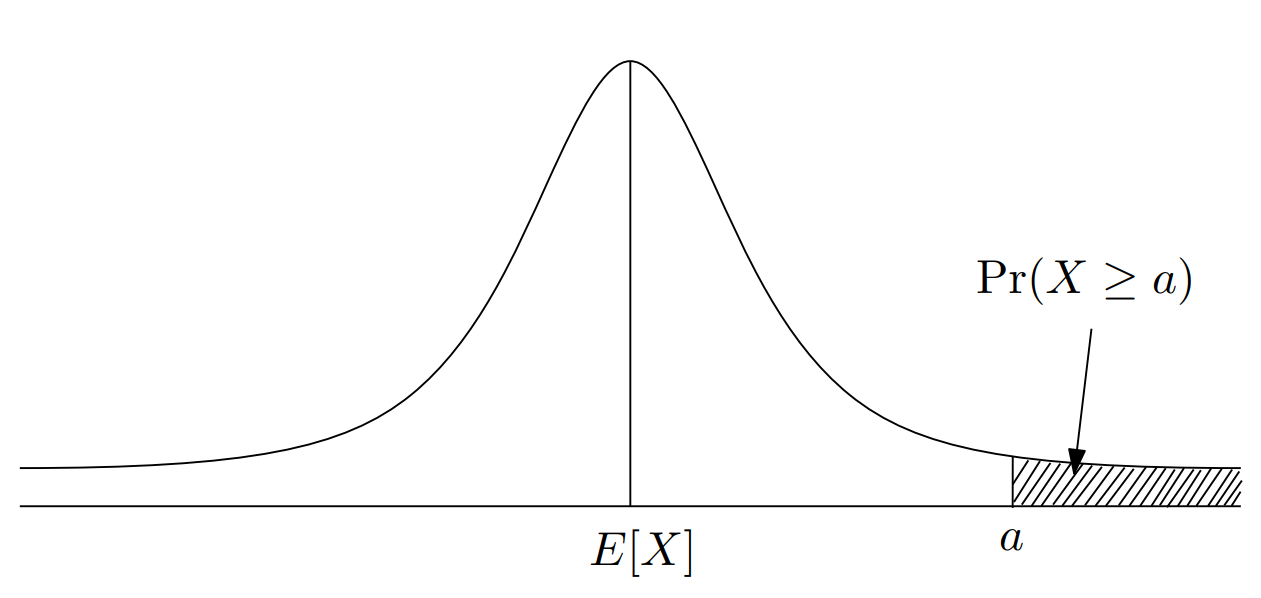
\includegraphics[width=0.7\textwidth]{img/markovbound.png}
    \caption{Markov's inequality bounds the probability for the shaded region $\mathbb{P}[X\geq a]$}
\end{figure}
\begin{proof}
    The proof is straightforward: \begin{equation}
        \begin{split}
            \mathbb{P}(Y\geq t) & = \mathbb{E}[\mathbbm{1}_{(Y\geq t)}]\\
            & \leq \frac{\mathbb{E}[Y\mathbbm{1}_{(Y\geq t)}]}{t}\\
            & \leq \frac{\mathbb{E}[Y]}{t}
        \end{split}
    \end{equation}
    We use the fact that\begin{equation}
        \mathbb{P}(Y\in A) = \int_{A} P_{Y} (dy) = \int_{Y} \mathbbm{1}_{(x\in A)} P_{Y}(dy) = \mathbb{E}[\mathbbm{1}_{Y\in A}]
    \end{equation}
    Additionally, we also have $Y\geq t > 0$ implies $Y/t \geq 1$, and $Y\geq 0\implies Y \mathbbm{1}_{(Y\geq t)}\leq Y$ which implies their expected value.
\end{proof}

If $\phi$ denotes a nondecreasing and nonnegative function defined on a possibly infinite interval $I\subset \mathbb{R}$, and if $Y$ denotes a random variable taking values in $I$, then Markov's inequality implies that for every $t\in I$ with $\phi(t)\neq 0$, 
\begin{equation}
    \mathbb{P} (Y\geq t) \leq \sP [\phi(Y)\geq \phi(t)] \leq \frac{\mathbb{E}[\phi(Y)]}{\phi(t)}
\end{equation}
This can be used to derive the Chebyshev's inequality later. 
\subsection{Chebyshev's inequality}
The common application of Markov's probability is Chebyshev's probability. Let $X$ be an arbitrary real random variable. Then for any $t> 0$, 
\begin{equation}
    \mathbb{P}(|X-\mathbb{E}[X]| \geq t) \leq \frac{\mathrm{Var}[X]}{t^{2}} 
\end{equation}
Where $\mathrm{Var}[X]:= \mathbb{E}[|X-\mathbb{E}X|^{2}]=\mathbb{E}[X^{2}]- (\mathbb{E}[X])^{2}$ is the variance of $X$. The prominent role of Chebyshev's inequality is not only explained by historical reasons, but also among all the absolute moments of the form $\mathbb{E}[|Z-\mathbb{E}(Z)|^{q}]$, the variance is typically the easiest to handle. 
\begin{proof}
    Let $X$ be a random variable, so $(X-\mathbb{E}[X])^{2}$ is a non-negative random variable. Hence, we can apply Markov's inequality: 
    \begin{align}
        \mathbb{P}(X-\mathbb{E}[X]\geq t) & = \mathbb{P}\left((X-\mathbb{E}[X])^{2}\geq t^{2}\right)\\
        & \leq \frac{1}{t^{2}} \mathbb{E} \left[(X-\mathbb{E}[X])^{2}\right]\\
        & = \frac{1}{t^2} \mathrm{Var}[X]
    \end{align}
\end{proof}
The property of Chebyshev's inequality contains several constraints, though arguably better than Markov's. Chebyshev's inequality does not require that the random variable is non-negative. However, it also requires that we know the variance in addition to the mean. Hence, the goal of Chebyshev's inequality is to bound the probability that the RV is far from its mean in either direction. While in principle Chebyshev's inequality asks about distance from the mean in either direction, it can still be used to give a bound on how often a random variable can take large values, and will usually give much better bound than Markov's inequality - since we have more knowledge of the distribution. 

We can use Chebyshev's inequality to prove a soft variation of the law of large number, or the \textit{weak law of large number}. 
\begin{theorem}[Week Law of Large Number]
    Let $X_{1},\dots,X_{n}$ be a sequence of i.i.d. random variables with mean $\mu$. Let $\bar{X}_{n}=(1/n)\sum_{i=1}^{n}X_{i}$ be the sample mean. Then $\bar{X}_{n}$ converges in probability to $\mu$. That is, for any $\epsilon>0$, 
    \begin{equation}
        \lim_{n\to\infty}\mathbb{P}\left(\lvert \bar{X}_{n}-\mu\rvert > \epsilon\right)=0
    \end{equation}
\end{theorem}
\begin{proof}
    By the property of the expectation and variance of sample mean consisting of $n$ i.i.d. variables, for $\mathbb{E}[\bar{X}_{n}]=\mu$ and $\mathrm{Var}(\bar{X}_{n})=\sigma^{2}/n$. By Chebyshev's inequality, 
    \begin{equation}
        \lim_{n\to\infty} \mathbb{P}\left(\lvert \bar{X}_{n}-\mu\rvert > \epsilon\right) \leq \lim_{n\to \infty} \frac{\mathrm{Var}(\bar{X}_{n})}{\epsilon^{2}} = \lim_{n\to\infty} \frac{\sigma}{n\epsilon^{2}} = 0
    \end{equation}
\end{proof}
\subsection{McDiarmid's inequality}
A generalization of Hoeffding's inequality is the McDiarmid's, or Bounded Difference inequality, where the quantity of interest is some function of the data, i.e. $S_{n}= \phi(X_{1},\dots,X_{n})$. Some restrictions on $\phi$ are required to get exponential bounds. 
\begin{theorem}[McDiarmid's Inequality]
    Let $X_{1},\dots,X_{n}$ be independent random variables, where $X_{i}$ has range $\mathcal{X}_{i}$. Let $f:\mathcal{X}_{1}\times \dots \times \mathcal{X}_{n}\to \mathbb{R}$ be any function with the $(c_1, \dots, c_{n})$-bounded difference property: for every $i=1,\dots,n$ and every $(x_1,\dots,x_n),(x_{1}',\dots,x_{n}')\in \mathcal{X}_{1}\times \dots\times \mathcal{X}_{n}$ that differ only in the $i$-th coordinate, we have: \begin{equation}
        \lvert f(x_1,\dots,x_n) - f(x_{1}',\dots,x_{n}') \rvert \leq c_{i}
    \end{equation}
    For any $t>0$: 
    \begin{equation}
        \mathbb{P}\Big([f(X_{1},\dots,X_{n})] - \mathbb{E}[f(X_{1},\dots,X_{n})]\geq t\Big) \geq \exp{\left(-\frac{2t^{2}}{\sum_{i=1}^{n}c_{i}^{2}}\right)}
    \end{equation}
\end{theorem}
\begin{proof}
    Write $\mathbb{E}_i[\cdot]$ to denote expectation conditioned on $X_{1:i} := (X_1, \ldots, X_i)$. Therefore, $g_i(X_{1:i}) := \mathbb{E}_i[f(X_{1:n})]$ is, as the notation suggests, a function of $X_{1:i}$. Now define the following random variables:
\[
Y_i := g_i(X_{1:i}) - g_{i-1}(X_{1:i-1}),
\]
\[
A_i := \inf_{x_i \in \mathcal{X}_i} g_i(X_{1:i-1}, x_i) - g_{i-1}(X_{1:i-1}),
\]
\[
B_i := \sup_{x_i \in \mathcal{X}_i} g_i(X_{1:i-1}, x_i) - g_{i-1}(X_{1:i-1}).
\]

These random variables satisfy
\[
Y_i \in [A_i, B_i], \quad \mathbb{E}_{i-1}[Y_i] = 0,
\]
\[
\sum_{i=1}^n Y_i = f(X_{1:n}) - \mathbb{E}[f(X_{1:n})].
\]

Furthermore, we claim that $[A_i, B_i]$ is always an interval of length at most $c_i$. We defer the proof of this claim to later.  

To bound the probability that the sum of the $Y_i$'s is at least $t$, we use the Chernoff bounding method. Let $S_i := Y_1 + \cdots + Y_i$. Then
\begin{align}
    \mathbb{E}[\exp(\lambda S_n)] 
    &= \mathbb{E}[\exp(\lambda(Y_n + S_{n-1}))] \\
    &= \mathbb{E}[\mathbb{E}_{n-1}[\exp(\lambda Y_n)] \exp(\lambda S_{n-1})]\\
    &\leq \exp(\lambda^2 c_n^2/8)\,\mathbb{E}[\exp(\lambda S_{n-1})]\\
    &= \exp(\lambda^2 c_n^2/8)\,\mathbb{E}[\exp(\lambda(Y_{n-1}+S_{n-2}))]\\
    &= \exp(\lambda^2 c_n^2/8)\,\mathbb{E}[\mathbb{E}_{n-2}[\exp(\lambda Y_{n-1})]\exp(\lambda S_{n-2})]\\
    &\leq \exp(\lambda^2 c_n^2/8)\exp(\lambda^2 c_{n-1}^2/8)\,\mathbb{E}[\exp(\lambda S_{n-2})]\\
    & \vdots \\
    &\leq \exp(\lambda^2 c_n^2/8)\cdots\exp(\lambda^2 c_1^2/8) \\
    &= \exp\left(\frac{\sum_{i=1}^n c_i^2}{4}\cdot\frac{\lambda^2}{2}\right).
\end{align}

Above, the inequalities all follow from Hoeffding's inequality. Therefore, $S_n$ is $\sum_{i=1}^n c_i^2/4$ sub-Gaussian. The probability bound now follows from the Cramer-Chernoff inequality for subgaussian random variables.

It remains to prove that $[A_i, B_i]$ is an interval of length at most $c_i$. We show that $B_i - A_i \leq c_i$. By independence of $X_1, \ldots, X_n$, we have

\begin{align}
g_i(X_{1:i-1}, x_i) 
&= \mathbb{E}[f(X_{1:i-1}, x_i, X_{i+1:n}) \mid X_{1:i-1}, X_i = x_i]   \\
&= \mathbb{E}[f(X_{1:i-1}, x_i, X'_{i+1:n}) \mid X_{1:i-1}],  
\end{align}
where $X'_{i+1:n}$ is an independent copy of $X_{i+1:n}$. Then
\begin{align}
B_i - A_i 
&= \sup_{b \in \mathcal{X}_i} g_i(X_{1:i-1}, b) - \inf_{a \in \mathcal{X}_i} g_i(X_{1:i-1}, a)   \\
&= \sup_{a,b \in \mathcal{X}_i} g_i(X_{1:i-1}, b) - g_i(X_{1:i-1}, a)  \\
&= \sup_{a,b \in \mathcal{X}_i} \mathbb{E}[f(X_{1:i-1}, b, X'_{i+1:n}) - f(X_{1:i-1}, a, X'_{i+1:n}) \mid X_{1:i-1}]   \\
&\leq \mathbb{E}\Big[\sup_{a,b \in \mathcal{X}_i} |f(X_{1:i-1}, b, X'_{i+1:n}) - f(X_{1:i-1}, a, X'_{i+1:n})| \,\Big|\, X_{1:i-1}\Big]   \\
&\leq c_i.  
\end{align}

The last step above uses the bounded differences property of $f$.
\end{proof}

\subsection{The Cramer-Chernoff method}
One more important bounding method that can be discussed in this section is the Cramer-Chernoff bound. This method determines the best possible bound for a tail probability that one can possibly obtain by using Markov's inequality with an exponential function $\phi(t)=\exp{(\lambda t)}$. This simple technique leads to surprisingly sharp bounds in many cases. We work out some simple examples, and then will proceed with some of its analytical properties. 

Let $Z$ be a real-valued random variable. For $\lambda\geq 0$, Markov's inequality implies 
\begin{equation}
    \sP [Z\geq t] \leq \exp{(-\lambda t)}\mathbb{E}[\exp{(\lambda Z)}]
\end{equation}
Since this inequality holds for all values of $\lambda \geq 0$, one may choose $\lambda$ to minimize the upper bound. Defining the logarithm of the moment generating function as 
\begin{equation}
    \phi_{Z}(\lambda) = \log{(\mathbb{E}[\exp{(\lambda Z)}])}, \quad \forall \lambda \geq 0 
\end{equation}
and introducing the supremum of such generating function being \begin{equation}
    \phi_{Z}^{*}(t) = \sup_{\lambda\geq 0}(\lambda t - \phi_{Z}(\lambda))
\end{equation}
We obtain the Chernoff's inequality:\index{Chernoff's inequality} 
\begin{equation}
    \sP [Z\geq t] \leq \exp{\left[-\left(\sup_{\lambda\geq 0}(\lambda t - \phi_{Z}(\lambda))\right)\right]} = \exp{[-\phi_{Z}^{*}(t)]}
\end{equation}
The function $\phi_{Z}^{*}(t)$ is called the \textit{Cramer transform} of $Z$. Usually, this is also called the Legendre transform (for example, in \cite{OstaszewskaZajkowski2014}) or Legendre-Fenchel transform. The Cramer transform is characterized of its shape by satisfying the \textit{Cramer's condition},\index{Cramer condition} 
\begin{definition}[Cramer's condition]
    Let $M_{X}$ denote the moment-generating function of a given random variable $X$, that is, $M_{X}(t)=\mathbb{E}[\exp{(tX)}]$. Then the random variable $X$ satisfies the \textit{Cramer condition} if there exists $c>0$ such that $\mathbb{E}[\exp{(|cX|)}]< \infty$. If $X$ satisfies the Cramer condition, then we call $M_{X}$ to be \textit{well-defined} (taking finite values) on a connected neighbourhood, containing the interval $[-c,c]$, of zero and moreover possess the expansion
    \begin{equation}
        M_{X}(t) = \sum^{\infty}_{n=0}\frac{\mathbb{E}[X^{n}]}{n!}t^{n}
    \end{equation}
    where $|t|<t_{0}$ and $t_{0}>c$. 
\end{definition}
The function itself is a nonnegative function, since $\phi_{Z}(0)=0$. If $\mathbb{E}[Z]$ exists, then the convexity of the exponential function and Jensen's inequality imply that $\phi_{Z}(\lambda)\geq \lambda \mathbb{E}[Z]$ and therefore, for all negative values of $\lambda$, $\lambda t - \phi_{Z}(\lambda)\leq 0$ whenever $t\leq \mathbb{E}[Z]$. This means that we may formally extend the supremum over all $\lambda \in \mathbb{R}$ of the Cramer transform, 
\begin{equation}
    \phi_{Z}^{*}(t) = \sup_{\lambda\in \mathbb{R}}(\lambda t - \phi_{Z}(\lambda))
\end{equation}
from this, formally, we treat the right-hand expression of the often known, as what we call the \textit{Fenchel-Legendre dual function} of $\phi_{Z}$. Thus, at every $t\geq \mathbb{E}[Z]$, the Cramer transform coincides with the Fenchel-Legendre dual. That is not to say they are the same, however the range of $\lambda$ is relevant. 